% ============================================================
% Chapitre 6 : Tests d'Hypotheses — Cadre General
% ============================================================
\chapter{Tests d'Hypoth\`eses --- Cadre G\'en\'eral}
\label{ch:tests}

\begin{center}
\textit{<<~L'absence de preuve n'est pas la preuve de l'absence.~>>} --- Carl Sagan
\end{center}

% ------------------------------------------------------------
\section{Exemple motivant}
% ------------------------------------------------------------

Un fabricant affirme que ses vis ont une r\'esistance moyenne de 50~kN. Un client pr\'el\`eve $n=25$ vis et mesure $\bar{x}=48{,}2$~kN avec $s=4{,}5$~kN. Cette diff\'erence est-elle significative ou simplement due au hasard de l'\'echantillonnage ?

% ------------------------------------------------------------
\section{Formulation des hypoth\`eses}
% ------------------------------------------------------------

\begin{definition}[Hypoth\`eses]
\index{hypothese nulle@hypoth\`ese nulle}\index{hypothese alternative@hypoth\`ese alternative}
\begin{itemize}
\item $H_0$ : \textbf{hypoth\`ese nulle} --- l'affirmation que l'on cherche \`a remettre en question.
\item $H_1$ : \textbf{hypoth\`ese alternative} --- ce que l'on soupçonne si $H_0$ est fausse.
\end{itemize}
Formes classiques pour un param\`etre $\theta$ :
\begin{center}
\begin{tabular}{lll}
\toprule
\textbf{Type} & $H_0$ & $H_1$ \\
\midrule
Bilat\'eral & $\theta=\theta_0$ & $\theta\neq\theta_0$ \\
Unilat\'eral gauche & $\theta\geq\theta_0$ & $\theta<\theta_0$ \\
Unilat\'eral droit & $\theta\leq\theta_0$ & $\theta>\theta_0$ \\
\bottomrule
\end{tabular}
\end{center}
\end{definition}

% ------------------------------------------------------------
\section{Erreurs de premi\`ere et deuxi\`eme esp\`ece}
% ------------------------------------------------------------

\begin{definition}[Types d'erreurs]
\index{erreur de type I}\index{erreur de type II}
\begin{center}
\begin{tabular}{l|cc}
& $H_0$ vraie & $H_0$ fausse \\
\hline
Rejeter $H_0$ & \textbf{Erreur de type I} ($\alpha$) & D\'ecision correcte \\
Ne pas rejeter $H_0$ & D\'ecision correcte & \textbf{Erreur de type II} ($\beta$) \\
\end{tabular}
\end{center}
\begin{itemize}
\item $\alpha = \Prob(\text{rejeter } H_0\mid H_0 \text{ vraie})$ : \textbf{niveau} (ou seuil) du test.
\item $\beta = \Prob(\text{ne pas rejeter } H_0\mid H_1 \text{ vraie})$.
\item $1-\beta$ : \textbf{puissance} du test.
\end{itemize}
\end{definition}

\begin{intuition}
$\alpha$ est le risque de <<~fausse alarme~>>. $\beta$ est le risque de <<~manquer~>> un vrai effet. En g\'en\'eral, on fixe $\alpha$ (souvent 5\%) et on cherche \`a maximiser la puissance.
\end{intuition}

% ------------------------------------------------------------
\section{Structure d'un test}
% ------------------------------------------------------------

\begin{definition}[Test statistique]
\index{test statistique}
Un \textbf{test} de $H_0$ contre $H_1$ au niveau $\alpha$ est une r\`egle de d\'ecision :
\begin{enumerate}
\item Calculer une \textbf{statistique de test} $T=T(X_1,\ldots,X_n)$.
\item D\'eterminer la \textbf{r\'egion critique} $W$ telle que $\Prob_{\theta_0}(T\in W)\leq\alpha$.
\item \textbf{D\'ecision} : rejeter $H_0$ si $T\in W$.
\end{enumerate}
\end{definition}

\begin{definition}[$p$-valeur]
\index{p-valeur@$p$-valeur}
La \textbf{$p$-valeur} est la probabilit\'e, sous $H_0$, d'observer une valeur de la statistique de test au moins aussi extr\^eme que celle observ\'ee :
\[
p = \Prob_{H_0}(T\geq t_{\mathrm{obs}}) \quad \text{(test unilat\'eral droit)}.
\]
On rejette $H_0$ si et seulement si $p\leq\alpha$.
\end{definition}

\begin{attention}
\textbf{La $p$-valeur n'est PAS} la probabilit\'e que $H_0$ soit vraie. C'est la probabilit\'e d'observer des donn\'ees aussi extr\^emes \textbf{si} $H_0$ \'etait vraie.

Autres pi\`eges :
\begin{itemize}
\item <<~$p>0{,}05$~>> ne signifie pas que $H_0$ est vraie, seulement que les donn\'ees ne fournissent pas de preuve suffisante contre $H_0$.
\item La significativit\'e statistique ($p<0{,}05$) n'implique pas la significativit\'e \textbf{pratique} (l'effet peut \^etre n\'egligeable).
\end{itemize}
\end{attention}

% ------------------------------------------------------------
\section{Puissance d'un test}
% ------------------------------------------------------------

\begin{definition}[Fonction puissance]
\index{puissance}
La \textbf{fonction puissance} du test est :
\[
\pi(\theta) = \Prob_\theta(\text{rejeter } H_0).
\]
\begin{itemize}
\item Pour $\theta\in\Theta_0$ (sous $H_0$) : $\pi(\theta)\leq\alpha$ (contr\^ole du niveau).
\item Pour $\theta\in\Theta_1$ (sous $H_1$) : $\pi(\theta)=1-\beta(\theta)$ (puissance).
\end{itemize}
Un bon test a une puissance \'elev\'ee pour les valeurs de $\theta$ sous $H_1$.
\end{definition}

\begin{center}
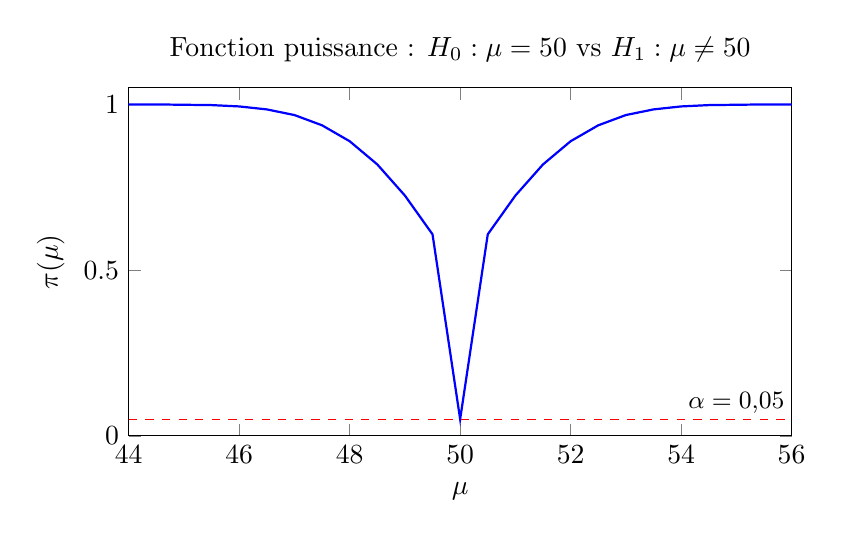
\begin{tikzpicture}
\begin{axis}[
    width=10cm, height=6cm,
    xlabel={$\mu$}, ylabel={$\pi(\mu)$},
    title={Fonction puissance : $H_0:\mu=50$ vs $H_1:\mu\neq 50$},
    xmin=44, xmax=56, ymin=0, ymax=1.05,
]
% Puissance tracee par points (normcdf n'existe pas dans pgfplots)
\addplot[thick,blue] coordinates {
(44,1.00)(44.5,1.00)(45,0.999)(45.5,0.998)(46,0.994)(46.5,0.985)
(47,0.968)(47.5,0.937)(48,0.889)(48.5,0.819)(49,0.725)(49.5,0.608)
(50,0.050)(50.5,0.608)(51,0.725)(51.5,0.819)(52,0.889)(52.5,0.937)
(53,0.968)(53.5,0.985)(54,0.994)(54.5,0.998)(55,0.999)(55.5,1.00)(56,1.00)
};
\addplot[dashed,red] coordinates {(44,0.05) (56,0.05)};
\node at (axis cs:55,0.1) {\small $\alpha=0{,}05$};
\end{axis}
\end{tikzpicture}
\end{center}

% ------------------------------------------------------------
\section{Lemme de Neyman--Pearson}
% ------------------------------------------------------------

\begin{theoreme}[Lemme de Neyman--Pearson]
\index{Neyman--Pearson}
\label{thm:neyman-pearson}
Pour tester $H_0:\theta=\theta_0$ contre $H_1:\theta=\theta_1$ (hypoth\`eses simples), le test le plus puissant de niveau $\alpha$ rejette $H_0$ lorsque le \textbf{rapport de vraisemblance} est grand :
\[
\Lambda(\mathbf{x}) = \frac{L(\theta_1;\mathbf{x})}{L(\theta_0;\mathbf{x})} > k_\alpha,
\]
o\`u $k_\alpha$ est choisi tel que $\Prob_{\theta_0}(\Lambda>k_\alpha)=\alpha$.
\end{theoreme}

\begin{proof}[Esquisse de preuve]
Soit $\varphi$ la r\`egle du test NP et $\varphi'$ tout autre test de niveau $\leq\alpha$. On veut montrer $\E_{\theta_1}[\varphi]\geq\E_{\theta_1}[\varphi']$.

Sur la r\'egion de rejet NP : $\varphi=1$, $L(\theta_1)\geq k\cdot L(\theta_0)$. Donc $(\varphi-\varphi')(L(\theta_1)-kL(\theta_0))\geq 0$ partout (les deux facteurs ont le m\^eme signe). En int\'egrant :
\[
\E_{\theta_1}[\varphi-\varphi'] \geq k\,\E_{\theta_0}[\varphi-\varphi'] = k(\alpha-\alpha')\geq 0. \qedhere
\]
\end{proof}

% ------------------------------------------------------------
\section{Test du rapport de vraisemblance g\'en\'eralis\'e}
% ------------------------------------------------------------

\begin{definition}[TRV g\'en\'eralis\'e]
\index{rapport de vraisemblance}
Pour $H_0:\theta\in\Theta_0$ contre $H_1:\theta\in\Theta_1=\Theta\setminus\Theta_0$, la statistique du \textbf{test du rapport de vraisemblance} (TRV) est :
\[
\lambda(\mathbf{x}) = \frac{\sup_{\theta\in\Theta_0} L(\theta;\mathbf{x})}{\sup_{\theta\in\Theta} L(\theta;\mathbf{x})}, \qquad 0\leq\lambda\leq 1.
\]
On rejette $H_0$ pour $\lambda\leq c_\alpha$ (petites valeurs de $\lambda$).
\end{definition}

\begin{theoreme}[Th\'eor\`eme de Wilks]
\index{Wilks}
Sous $H_0$ et des conditions de r\'egularit\'e :
\[
-2\ln\lambda(\mathbf{X}) \xrightarrow{\mathcal{L}} \chi^2(r),
\]
o\`u $r=\dim(\Theta)-\dim(\Theta_0)$ est le nombre de contraintes impos\'ees par $H_0$.
\end{theoreme}

% ------------------------------------------------------------
\section{Impl\'ementation Python}
% ------------------------------------------------------------

\begin{python}
\begin{minted}{python}
import numpy as np
from scipy import stats

# --- Test sur la moyenne (sigma inconnu) ---
# H0: mu = 50, H1: mu != 50
data = np.array([48.2, 47.5, 49.1, 46.8, 50.3, 48.7, 47.9, 49.5,
                 46.2, 48.8, 49.0, 47.3, 48.1, 50.1, 47.0,
                 49.4, 48.6, 46.5, 49.8, 47.2, 48.3, 49.7,
                 47.8, 48.5, 46.9])
n = len(data)
mu0 = 50
xbar = np.mean(data)
s = np.std(data, ddof=1)
t_obs = (xbar - mu0) / (s / np.sqrt(n))
p_value = 2 * stats.t.cdf(t_obs, df=n-1)  # bilateral, t_obs < 0
print(f"t_obs = {t_obs:.4f}, p-valeur = {p_value:.6f}")

# Avec scipy
t_stat, p_val = stats.ttest_1samp(data, mu0)
print(f"scipy: t = {t_stat:.4f}, p = {p_val:.6f}")

if p_val < 0.05:
    print("Conclusion: on rejette H0 au niveau 5%.")
else:
    print("Conclusion: on ne rejette pas H0 au niveau 5%.")

# --- Calcul de puissance ---
from scipy.stats import norm

def power_z_test(mu_true, mu0, sigma, n, alpha=0.05):
    """Puissance d'un test z bilateral."""
    z_alpha = norm.ppf(1 - alpha/2)
    delta = (mu_true - mu0) / (sigma / np.sqrt(n))
    power = 1 - norm.cdf(z_alpha - delta) + norm.cdf(-z_alpha - delta)
    return power

mu_values = np.linspace(44, 56, 200)
powers = [power_z_test(mu, 50, 4.5, 25) for mu in mu_values]

import matplotlib.pyplot as plt
plt.figure(figsize=(8, 5))
plt.plot(mu_values, powers, 'b-', lw=2)
plt.axhline(0.05, color='red', linestyle='--', label=r'$\alpha=0.05$')
plt.axvline(50, color='gray', linestyle=':')
plt.xlabel(r'$\mu$ (vraie valeur)')
plt.ylabel(r'$\pi(\mu)$ (puissance)')
plt.title('Fonction puissance du test z bilateral')
plt.legend()
plt.savefig("ch06_puissance.pdf")
plt.show()

# --- Taille d'echantillon pour puissance cible ---
def sample_size_z(mu_alt, mu0, sigma, alpha=0.05, power=0.8):
    z_alpha = norm.ppf(1 - alpha/2)
    z_beta = norm.ppf(power)
    n = ((z_alpha + z_beta) * sigma / (mu_alt - mu0))**2
    return int(np.ceil(n))

n_needed = sample_size_z(48, 50, 4.5)
print(f"Taille pour detecter mu=48 avec puissance 80%: n = {n_needed}")
\end{minted}
\end{python}

% ------------------------------------------------------------
\section{Exercices}
% ------------------------------------------------------------

\begin{exercice}[$\star$ -- Test de base]
Un enseignant affirme que la note moyenne est 12. Sur 20 copies, on observe $\bar{x}=11{,}2$ et $s=2{,}5$. Tester $H_0:\mu=12$ vs $H_1:\mu<12$ au niveau 5\%.
\end{exercice}

\begin{exercice}[$\star\star$ -- Neyman--Pearson]
Soit $X_1,\ldots,X_n\iid\mathcal{N}(\mu,1)$. Appliquer le lemme de Neyman--Pearson pour $H_0:\mu=0$ vs $H_1:\mu=1$. En d\'eduire la r\'egion critique optimale.
\end{exercice}

\begin{exercice}[$\star\star$ -- Puissance]
Pour le test $H_0:\mu=100$ vs $H_1:\mu\neq 100$ avec $\sigma=15$ et $\alpha=0{,}05$ :
\begin{enumerate}
\item Calculer la puissance pour $n=25$ et $\mu_1=105$.
\item Quelle taille d'\'echantillon faut-il pour une puissance de 90\% \`a $\mu_1=105$ ?
\end{enumerate}
\end{exercice}

\begin{exercice}[$\star\star$ -- TRV]
$X_1,\ldots,X_n\iid\mathcal{N}(\mu,\sigma^2)$ avec $\sigma^2$ inconnu. Calculer $\lambda$ pour $H_0:\mu=\mu_0$ et montrer que $-2\ln\lambda$ est une fonction croissante de $|T|$ o\`u $T$ est la statistique de Student.
\end{exercice}

\begin{exercice}[$\star\star\star$ -- Projet : simulations de puissance]
Pour le test $t$ unilat\'eral, \'etudier par simulation : (a) le taux d'erreur de type I pour diff\'erentes distributions (normale, exponentielle, uniforme), (b) la puissance en fonction de la taille d'effet $\delta=(\mu_1-\mu_0)/\sigma$, (c) comparer la puissance du test $t$ et du test de Wilcoxon.
\end{exercice}

% ------------------------------------------------------------
\begin{formules}
\begin{align*}
\alpha &= \Prob(\text{rejeter } H_0\mid H_0) & \beta &= \Prob(\text{ne pas rejeter } H_0\mid H_1) \\
p\text{-valeur} &= \Prob_{H_0}(T\geq t_{\mathrm{obs}}) & \pi(\theta) &= \Prob_\theta(\text{rejeter}\ H_0) \\
\text{NP} &: \text{rejeter si } \frac{L(\theta_1)}{L(\theta_0)}>k_\alpha &
\lambda &= \frac{\sup_{\Theta_0}L}{\sup_\Theta L}
\end{align*}
Wilks : $-2\ln\lambda\xrightarrow{\mathcal{L}}\chi^2(r)$.
\end{formules}
